\documentclass[11pt]{article}
\usepackage{epsfig,psfrag}
\usepackage{amsmath}

\setlength{\textwidth}{6.2in}
\setlength{\oddsidemargin}{0.3in}
\setlength{\evensidemargin}{0in}
\setlength{\textheight}{8.7in}
\setlength{\voffset}{-.7in}
\setlength{\headsep}{26pt}
\setlength{\parindent}{10pt}
\begin{document}


% a few handy macros

\newcommand\matlab{{\sc matlab}}
\newcommand{\goto}{\rightarrow}
\newcommand{\bigo}{{\mathcal O}}
\newcommand{\half}{\frac{1}{2}}
%\newcommand\implies{\quad\Longrightarrow\quad}
\newcommand\reals{{{\rm l} \kern -.15em {\rm R} }}
\newcommand\complex{{\raisebox{.043ex}{\rule{0.07em}{1.56ex}} \hskip -.35em {\rm C}}}


% macros for matrices/vectors:

% matrix environment for vectors or matrices where elements are centered
\newenvironment{mat}{\left[\begin{array}{ccccccccccccccc}}{\end{array}\right]}
\newcommand\bcm{\begin{mat}}
\newcommand\ecm{\end{mat}}

% matrix environment for vectors or matrices where elements are right justifvied
\newenvironment{rmat}{\left[\begin{array}{rrrrrrrrrrrrr}}{\end{array}\right]}
\newcommand\brm{\begin{rmat}}
\newcommand\erm{\end{rmat}}

% for left brace and a set of choices
\newenvironment{choices}{\left\{ \begin{array}{ll}}{\end{array}\right.}
\newcommand\when{&\text{if~}}
\newcommand\otherwise{&\text{otherwise}}
% sample usage:
%  \delta_{ij} = \begin{choices} 1 \when i=j, \\ 0 \otherwise \end{choices}


% for labeling and referencing equations:
\newcommand{\eql}{\begin{equation}\label}
\newcommand{\eqn}[1]{(\ref{#1})}
% can then do
%  \eql{eqnlabel}
%  ...
%  \end{equation}
% and refer to it as equation \eqn{eqnlabel}.  


% some useful macros for finite difference methods:
\newcommand\unp{U^{n+1}}
\newcommand\unm{U^{n-1}}

% for chemical reactions:
\newcommand{\react}[1]{\stackrel{K_{#1}}{\rightarrow}}
\newcommand{\reactb}[2]{\stackrel{K_{#1}}{~\stackrel{\rightleftharpoons}
   {\scriptstyle K_{#2}}}~}

  % input some useful macros

% Macros for exercises:

\newcommand{\exernum}{0.0} % will be set to current Exercise number

% Headers:

\newcommand{\exercise}[2][\null]{\vskip 15pt \noindent%
     {\large \bf Exercise #2}~ {\it #1}%
     \nopagebreak\vskip 5pt \nopagebreak%
     \renewcommand{\exernum}{#2} \setcounter{equation}{0}%
     \addcontentsline{toc}{subsection}{Exercise #2 \hskip 5pt #1}}
     % \exercise has optional first argument -- short descriptor
     % the exercise number is stored in \exernum for use in labeling equations

\newcommand{\chapexercises}[1]{%
     \cleardoublepage
     \centerline{\LARGE\bf Chapter #1 Exercises}
     \vskip .5cm
     \noindent
     From: {\it Finite Difference Methods for Ordinary and Partial 
     Differential Equations}\\  by R.~J.~LeVeque, SIAM, 2007.~~~
     {\tt http://www.amath.washington.edu/$\sim$rjl/fdmbook}
     \vskip .5cm
     \addcontentsline{toc}{section}{Chapter #1}
     }

% Parts:

% set enumerate to give parts a, b, c, ...  rather than numbers 1, 2, 3...
\renewcommand{\theenumi}{\alph{enumi}}
\renewcommand{\labelenumi}{(\theenumi)}

% set second level enumerate to give parts i, ii, iii, iv, etc.
\renewcommand{\theenumii}{\roman{enumii}}
\renewcommand{\labelenumii}{(\theenumii)}

% Equations:

% label equations starting with E for exercise, then exernum, then a,b,c etc
\renewcommand{\theequation}{Ex\exernum\alph{equation}}


% commands for labeling and citing equations to add exernum automatically.
%   then set equations using e.g. \eqlex{a} ... \end{equation}
%   and cite as \eqnex{a}
\newcommand{\eqlex}[1]{\begin{equation}\label{\exernum #1}}
\newcommand{\eqnex}[1]{(\ref{\exernum #1})}
       % more macros for exercise formatting

% For exercises,
% set enumerate to give parts a, b, c, ...  rather than numbers 1, 2, 3...
\renewcommand{\theenumi}{\alph{enumi}}
\renewcommand{\labelenumi}{(\theenumi)}


% header:
\chapexercises{4}


\exercise[(Convergence of SOR)]{4.1}

The m-file \verb+iter_bvp_Asplit.m+ implements the Jacobi, Gauss-Seidel, and
SOR matrix splitting methods on the linear system arising from the boundary
value problem $u''(x) = f(x)$ in one space dimension.  

\begin{enumerate}
\item Run this program for each method and produce a plot similar to 
Figure~4.2.

\item The convergence behavior of SOR is very sensitive to the choice of
$\omega$ ({\tt omega} in the code).  Try changing from the optimal $\omega$
to $\omega = 1.8$ or 1.95.

\item Let $g(\omega) = \rho(G(\omega))$ be the spectral radius of the
iteration matrix $G$ for a given value of $\omega$.  Write a program to
produce a plot of $g(\omega)$ for $0\leq \omega \leq 2$.

\item From equations (4.22) one might be tempted to try to implement SOR as
\begin{verbatim}
     for iter=1:maxiter
        uGS = (DA - LA) \ (UA*u + rhs);
        u = u + omega * (uGS - u);
        end
\end{verbatim}
where the matrices have been defined as in \verb+iter_bvp_Asplit.m+.
Try this computationally and observe that it does not work well.  Explain
what is wrong with this and derive the correct expression (4.24).

\end{enumerate} 


\exercise[(Forward vs.\ backward Gauss-Seidel)]{4.2}

\begin{enumerate}
\item The Gauss-Seidel method for the discretization of $u''(x) = f(x)$
takes the form (4.5) if we assume we are marching forwards across the grid,
for $i=1,~2,~\ldots,~m$.  We can also define a {\it backwards Gauss-Seidel
method} by setting
\eqlex{a}
u_i^{[k+1]} = \half (u_{i-1}^{[k]} + u_{i+1}^{[k+1]} - h^2 f_i), \qquad
\text{for}~ i = m,~m-1,~m-2,~\ldots,~1.
\end{equation}
Show that this is a matrix splitting method of the type described in
Section~4.2 with $M = D-U$ and $N=L$.

\item Implement this method in \verb+iter_bvp_Asplit.m+ and observe that it
converges at the same rate as forward Gauss-Siedel for this problem.

\item Modify the code so that it solves the boundary value problem
\eqlex{b}
\epsilon u''(x) = au'(x) + f(x),\qquad 0\leq x \leq 1,
\end{equation} 
with $u(0) = 0$ and $u(1) = 0$, where $a\geq 0$ and the $u'(x_i)$ term
is discretized by the one-sided approximation $(U_i - U_{i-1})/h$.
Test both forward and backward Gauss-Seidel for the resulting linear system.
With $a=1$ and $\epsilon = 0.0005$.  You should find that they behave very
differently:

\psfrag{forwardGS}{forward}
\psfrag{backwardGS}{backward}
\hfil\epsfig{file=figs/iter_bvp_advdiff.eps,width=3.5in}\hfil

Explain intuitively why sweeping in one direction works so much better than
in the other.

{\bf Hint:} Note that this equation is the steady equation for an 
advection-diffusion
PDE $u_t(x,t) + au_x(x,t) = \epsilon u_{xx}(x,t) - f(x)$.  
You might consider how the methods behave in the case $\epsilon = 0$.
\end{enumerate} 


\end{document}


